\documentclass[letterpaper, 11 pt, conference]{article}
\usepackage{graphicx}
\usepackage{lipsum}
\usepackage{verbatim}
\usepackage{listings}
\usepackage{rotating}
\usepackage[titletoc]{appendix}
\usepackage[left=2.5cm,top=3cm,right=2.5cm,bottom=3cm,bindingoffset=0.5cm]{geometry}
\title{\Huge \textbf{Duck Hunt and CPU }} 
\author{Phillip Bradbury, Zach Toolson, Dan Willoughby}

\begin{document}
\maketitle
\clearpage

\tableofcontents
\clearpage
\begin{abstract}
  The CPU detailed in this report uses a modified CR-16 architecture which can interface with two NES-compatible Light Guns and a VGA compatible display.  The CPU can interface with the Light Guns and the Picture Processing Unit via memory-mapped I/O.  The Light Guns require a CRT-based VGA display to function fully with the Rubber Duck Hunt program included in the Plan B archive.

\end{abstract}

\section{Introduction}
The purpose of this project is to create and detail the implementation of a CR-16 processor with a dedicated Picture Processing Unit and interfaces with NES compatible Light Guns with the final goal of playing two-player competitive Rubber Duck Hunt on a CRT Display.  The Picture Processing Unit contains two fully distinct 80x60 character-based glyph maps with a dedicated debug screen which details the current state of the CPU's execution.  Additionally, the Picture Processing Unit provides a single hardware sprite capable of being rendered in three bits of color with 1 alpha bit for transparency.

The final CPU is a multi-cycle design with most operations taking 3 cycles, and LOAD and STOR operations requiring 4 cycles.  While the system is stable at 50MHz, the CPU is set to run at 142.8kHz to make counting 1/60th of a second frames easier and for smoother sprite movement.  Instruction and Data memory is a unified 16,384x18-bit block RAM providing full access to the instruction memory for programs that require run-time modifications.
\begin{center}
\begin{figure}
\caption{Schematic of CPU}
\makebox[\textwidth]{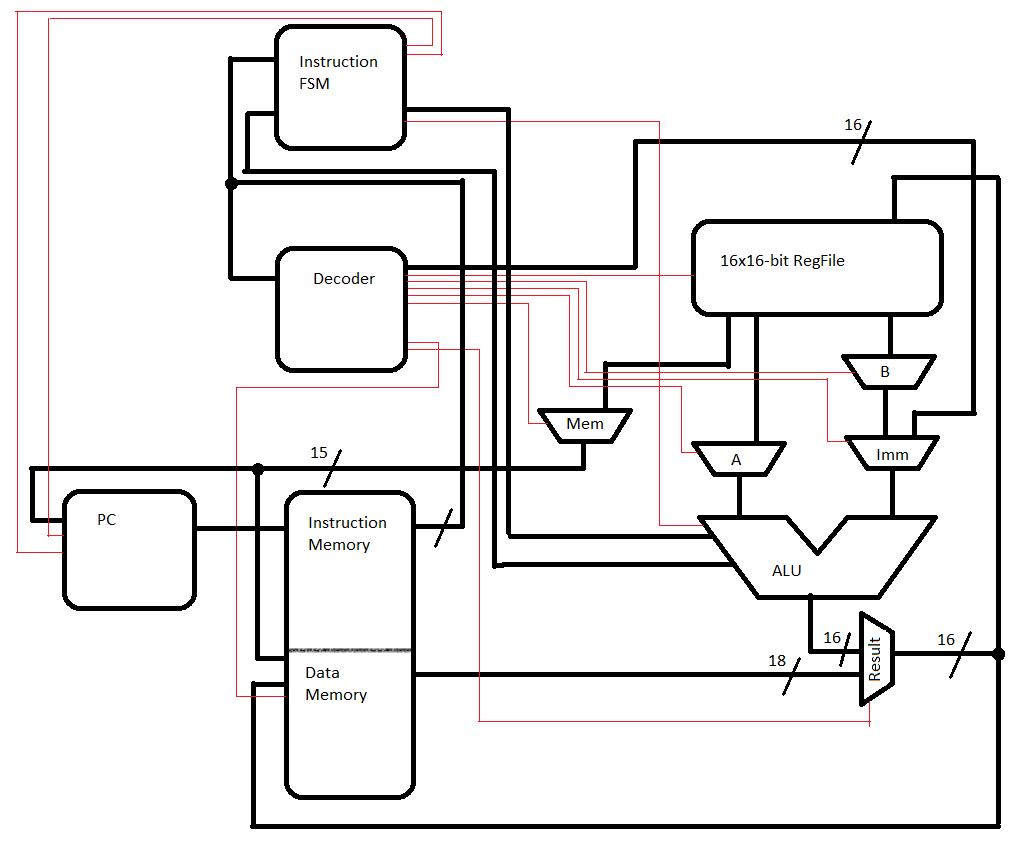
\includegraphics[width=\paperwidth]{cpu.png}}
\label{fig:schematic}
\end{figure} 
\end{center} 



\section{Picture Processing Unit}

The primary output of the CPU is to a VGA interface.  VGA is an extremely simple sequential state machine generated using the guidelines in the Nexys 3 Reference Manual.  The VGA interface sets an HSYNC and a VSYNC signal to tell the display when to reset the horizontal scan and the vertical scan respectively, and writes the 8-bit RGB value generated by either the Pixel Generator or the Sprite Generator modules.

The Picture Processing Unit accepts STOR commands when address[15:14] is 2'b11.  The bottom three bits of the address determine which property of the VGA interface is being modified as shown below.

000: HLocation1 - 10-bit Horizontal position of the first sprite pixel

001: VLocation1 - 10-bit Vertical position of the first sprite pixel

010: displayBlack - Boolean for whether the display should be set to black

011: displayColor - 8-bit color value for the background

100: sprite1On - Boolean for whether the sprite should be displayed or not

101: sprite1White - Boolean for whether the sprite should be overwritten with white pixels

110: textColor - 8-bit color value for the characters.

In the final iteration of the Picture Processing Unit, an additional clock was generated to produce a 4 second period blinking light as an input to several special Christmas light glyphs.

The VGA Controller also determines where the sprite is currently located on the display and either draws the sprite overlaid on the glyph map if the alpha boolean generated by the Sprite Generator module is true or displays the underlying glyphs if it is false.

Additional inputs to the Picture Processing Unit are passed to the Sprite Generator and the Pixel Generator modules.

\subsection{Pixel Generator}

The Pixel Generator is the most complex module in the display interface and controls the primary display.  The current pixel RGB information is stored in a character-based glyph map which is contained in a block RAM.  Each 8x8 pixel block of the 640x480 pixel display is stored in a 6-bit value, meaning that 3 total glyphs are stored per memory address with an offset of 0, 6, or 12 to obtain the currently displayed glyph.  Each glyph is stored in 4 memory addresses with two lines per address and 1-bit color.  If the current bit is a 1, then the Pixel Generator will return an 8-bit value for the text color--similarly, if the current bit is a 0, then the Pixel Generator will return an 8-bit value for the display color.

The glyph map allows 80x60 characters to be displayed on screen with a default glyph of the space character which displays only the background color.  Additional glyph code information can be found in the 'fake ascii.txt' file in the main project archive.  In general, alphanumeric and punctuation symbols are between 1-41, with all special glyph codes occurring between 42-63.

The Pixel Generator accepts STOR instructions when the address[15:14] is 2'b10.  Using this functionality, the glyph map can be partially accessed by the CPU.  Since memory is accessed in three glyph chunks, however, this is not the most effective way of writing data to the glyphmap.  The preferred method is to use a GSTOR instruction, which 3 registers--one to store the address, and two to store all 18-bits of data to be written to the address.

The glyph map used by the Pixel Generator for normal operation is located within addresses 1620 and 3239 in the video memory module.  This memory module is separate from the main instruction/data memory due to read/write port limitations.  Since the characters are stored using a six-bit encoding for space limitations, the data for the characters is stored in a 1024x18bit block RAM that is initialized on programming the FPGA.  While this memory is essentially read-only, using the block RAM frees up LUTs for later expansion, which proved to be invaluable as the pixel generator increased in complexity.  The block RAMs introduced a problem which is still unsolved--a delay in reading from the block RAMs as the pixels are being generated which creates a slight blur due to the pixel clock not being as precise as a 640x480 display requires.

The Pixel Generator also retrieves most pertinent information from the CPU as instructions are being executed.  This includes the entire register file, the program counter, inputs to the ALU, outputs from the ALU and data memory, and the current instruction being executed.  This information is used by the Pixel Generator to create a Debug Screen.

\subsection{Debug Screen}

The Debug Screen is located between addresses 0 and 1619 in the glyph map and pulls information directly from the CPU as it executes and writes the information to the Debug glyph map addresses in hardcoded locations so that if the Debug boolean--set by external switch--is true, the display ignores the sprite and displays the state of the CPU.  All values, including register selections, are displayed in hexadecimal to avoid conversions within the VGA module as this would introduce unnecessary delay.  This screen is especially effective in the Pause mode, where single-stepping through an assembled program can reveal underlying problems with the program design as well as with the primary hardware design.  Utilizing this functionality, we discovered a fatal flaw in the instructionFSM module:  we were capturing the ALU flags during decode, when they were being overwritten by the decoded instruction.  With a simple modification, the instructionFSM was capturing the ALU flags at the end of any instruction's final phase, allowing full use of the BEQ, BNEQ, BLE, BLT, BGE, and BGT instructions.

Actual implementation of the debug screen requires an internal state machine which counts from one to 53.  Since most values being written are 16 bits in total, this requires 2 memory writes for these values and a single memory write for the register select signals.  Decoding the instruction into human readable form requires the same case statement as in the instruction decoder, and uses the same parameters -- making the logic trivial and the actual character encoding tedious, yet valuable.  We determined the hardcoded addresses of the debug portion of the glyph map by counting lines in the encoded glyph map memory file and determining the correct locations for each signal to be written.

\subsection{Sprite Generator}

The Sprite Generator module instantiates a ROM containing a pre-defined 64x64 pixel sprite image using a 4-bit alpha/color encoding.  Four pixels of information are stored per 18-bit word, with the first bit containing an alpha boolean used by the Picture Processing Unit module to either display the RGB value generated by the Sprite Generator, or to display the underlying glyph information.  The Sprite Generator uses a naive upscale method from 3-bit color to 8-bit color, but could easily be modified to accept any 3-bit color encoding desired for the sprite coloration.  The Sprite Generator could be improved in any number of ways, not the least of which would be: more sprites, ability to change sprite color encoding via CPU instruction, and ability to specify sprite size.



\section{Software}

\subsection{Data Representation}
\label{data_rep}

The assembly code required certain functionality such as pointers and variables. Since assembly code doesn’t really inherently have variables or pointers conventions were established to accomplish these tasks. The assembler was robust enough that is could load in labels as immediate values. The convention for labels are as follows:

\begin{itemize}
  \item Labels must start with a letter (A-Z or a-z)
  \item Label must end with a colon ( : )
  \item Labels are treated as immediates in assembly
\begin{itemize}
  \item Example:
\begin{itemize}
  \item movi MyLabel, \$1
  \item cmpi AnotherLabel, \$1
\end{itemize}
\end{itemize}
  \item All labels must be loaded with LBN (see pseudo instruction)
\end{itemize}


Having the convention for labels established, the convention for variables was established as:


\begin{itemize}
    \item A label reserves a variable's position in memory with a NOP
    \item All variables will start with VAR\_
    \item Example:
\begin{itemize}
    \item VAR\_myVar: xor \$0, \$0
\end{itemize}
\end{itemize}

For a variable to be loaded it required first that the address of the location (pointer) be read, then the contents stored at that address be loaded. Since variables, by convention, were labels it did not matter where a variable was declared. The convention allowed for many values to be loaded and stored into memory. As the assembly program grew in length, it soon required that a pseudo instruction be made to load in variables and labels ( when an immediate value exceeded 8 bits or the value 255 it required more than one instruction ). The issue with the labels being greater than 8 bit numbers was resolved through the following pseudo instruction:

\begin{itemize}
    \item LBN - Loads a 16-bit number into a register

\begin{itemize}
        \item LBN \$Rsrc, \$Rdest,

        \item Example:
\begin{itemize}
            \item LBN \$3, \$1, 0x1234
            \item LBN \$3, \$1, my\_label
\end{itemize}

        \item The assembler compiles it to 3 instructions
\begin{itemize}
            \item LBN \$3, \$1, 0x1234
\begin{itemize}
                \item LUI 0x12, \$1
                \item MOVI 0x34, \$3
                \item OR \$3, \$1
\end{itemize}
\end{itemize}
        \item All labels must be loaded with LBN

\end{itemize}
    \item NUM - initializes an immediate into memory (Useful for writing glyphs)
\begin{itemize}
        \item hex: NUM 0x123
        \item letters\_PLA: NUM 0b011010\_010110\_001011

        \item decimal: NUM 1234

        \item This is how you can load a letter:
\begin{itemize}
            \item P: NUM 0b011010
            \item LBN \$1, \$13, P
            \item load \$13, \$13
\end{itemize}
\end{itemize}

\end{itemize}


The LBN instruction was used for all labels and variables which ultimately gave the functionality of pointers and variables. 

\subsection{Function Calls}

Similar to pointers and variables, the function calls were accomplished entirely by convention. To create a “function”, a large comment was included above the first instruction that included the label of the method. In this large comment, the argument registers were specified. For example, most function calls required a return address so the comment would specify that register 12 was the address to be return to after completion. Other functions might have specified numbers of where the duck was to be drawn or which player score to increment. Using registers to pass arguments soon began to complicate the process of writing assembly code. In order to overcome this complication, a convention for the use of registers was established. The register convention decided upon was as follows:

\begin{itemize}
    \item 0-6 temp (0 used for nop's)
    \item 7-9 saved values ( if you really want to save something, just store it in memory)
    \item 10-14 argument
    \item 15 return value
\end{itemize}


The majority of the registers were used for either temporary purposes or for argument passing. Most values that needed to be saved off such as duck position or players score used a variable described in section \ref{data_rep}.

\subsection{Prototpye}

We approached the software design by first implementing the duck hunt game in ruby. The library used to implement the game was called ruby-game. Ruby-game took care of a lot of the backend functions such as drawing sprites to the screen and the movement of sprites. Using the abstraction we gained from ruby-game, it was easy to figure out the inner working of duck hunt. The goal was to have a working high level prototype of the game that could then later be translated to assembly code. Once the ruby game was finished, an outline was created in modified CR-16 assembly code. The outline included functions such as move duck, increment score, check gun sensor, check gun trigger, and turn off the background. The main purpose of the prototype in ruby helped establish which functions were required to be written in assembly.  With these functions in mind, they were then implement into the assembly code.

\subsection{Game Application}

The prototype established functionality that needed to be implemented in the duck hunt game. 

The main functionality of duck hunt was moving the duck around randomly. The algorithm used to establish the random movement was a state machine with four states. The first state would begin the game by generating random x and y coordinates which were then passed to the move duck function.  The move duck function would move the duck one pixel in both the x and y direction until it reached a specified coordinate. Once the coordinate was reached, the function would return to one of the four states. Each of the four states would generate a random coordinate for the duck to move to. The states were organized in such a way that each coordinate was in a specific range, guaranteeing that the duck would be on screen more than it was off screen. 

The memory mapper included a way to get random numbers from the hardware random number generator. The convention for getting a random number from the generator were as follows:

\begin{itemize}
    \item LBN \$0, \$1, 0x2008 \# 8bit random number
    \item LBN \$0, \$1, 0x2009 \# 9bit random number
    \item LBN \$0, \$1, 0x2010 \# 10bit random number
\end{itemize}


Once the duck was moving randomly, a function (called checkgun) needed to be implemented that allowed the player to shoot the duck. The first obstacle with  implementing this function was to read the gun output and display what was read to the player. A memory mapper was needed to interface the gun signals with memory. Once the memory mapper was completed, the gun signal could now be read in assembly using a load instruction. The duck hunt game was two player, so it required reading values from two guns but the concept is the same for both guns.

The gun functionality was achieved by reading the trigger first, blacking out the background, and then checking if the gun sensor for light. To achieve such as feat it required the use of many boolean variables. Instead of using multiple registers for these values, the booleans were assigned to different bits in a single register. The program would load each gun’s output as booleans into two separate registers. For example, the gun trigger would be the least significant bit and the gun sensor would be the next bit position to the left. Immediately after the gun trigger was pulled, the program notified the VGA to turn off the background. The VGA took some time to respond, so a sleep function needed to be installed. The sleep function was simply a while loop that would iterate for a specified amount of time.After returning from the sleep function, the gun sensor could be checked and stored into a register as a boolean. After gathering the gun signals, “if” statements were implemented that would assign points to a player that had true values for the gun trigger and gun sensor ( If the sensor was true, that meant the gun was pointed at the duck, since the background was turned off). If a player had hit a duck, the application would call the increment score function for that player. 

The remaining methods to implement were increment score and duck dies. The increment score method would load the corresponding player’s score variable, increment it by one, and then display that to the screen. The duck dies function had was a bit more involved than incrementing the score. The first step to the duck dies function was to immediately draw the duck off the screen, preventing players from shooting it. Then the function would change the background color based on which player had hit the duck so the player’s would know who actually killed the duck. The final action was to call the sleep function, to allow the VGA to update (aka draw the duck off screen). A mixture of all the functions allowed for duck hunt to be implemented fully.


\section{Gun}

The gun’s used for the duck hunt game were an NES game controller knock off. Each gun included a photodiode and a trigger which were active high. The guns required a pull up resistor, so we configured the pmod appropriately. Occasionally with one pull of the trigger, the gun would send multiple high signals. The problem was resolved by designing a button debouncing system in hardware which interfaces with the gun. Button debouncing waits an allocated amount of time before reading the signal again. The sensors for the gun had a similar problem in that it would send pulses instead of one solid signal. This problem was resolved by creating a state for the sensor in a module. After receiving a high signal from the sensor, the module would wait before resetting the signal back to low. The pulses from the gun sensor would keep the state high as long as the gun was sensing light. The gun module is initialized in a memory mapper that allows the software to read the gun signals.

The conventions established to read the gun signals with the memory mapper were as follows:

\begin{itemize}
    \item LBN \$0, \$3, 0x2000 \# player 1 trigger
    \item LBN \$0, \$3, 0x2001 \# player 1 sensor
    \item LBN \$0, \$3, 0x2002 \# player 2 trigger
    \item LBN \$0, \$3, 0x2003 \# palyer 2 sensor
\end{itemize}

Each of the wires from the gun that were connected to the pmod on the FPGA were as follows: 
\begin{itemize}
\item red is vcc
\item yellow ground
\item brown trigger
\item blue photo
\end{itemize}


\section{Music Box}

\subsection{Implementation}
To implement the music box, there were two modules written and designed. The first module is one that plays the note with the frequency of the note as an input. A counter was then used in the module based on the clock to allow a set amount of time before flipping the square wave.  This module then outputs a square wave in the desired frequency to a connected speaker playing the note. The other module was a state machine that controlled which note to play. This was designed based on a one second long whole note, with each state being the length of an 8th note. In order to celebrate the season when our presentation took place, the music played the popular winter song Jingle Bells.


\section{ALU}
\subsection{Design}
The ALU designed performs 16-bit integer operations on two inputs. Our ALU performs both addition, subtraction, comparison, logical, and shifting operations on unsigned and signed integers. We treat signed integers using the two’s complement numbers. Most of the design decision came when determining which specific operations we wanted to implement as well as defining what those operations will do. Table 1 shows a list of operations that our ALU implements, as well as each flag that is could possibly throw. Another design decision that we made was to include a carry bit as an input. This was done to make our carry addition and subtraction operations with a carry bit simpler. The inputs and outputs to the ALU are:
\begin{itemize}
\item Input: 1-bit carry 
\item Input: Two 16-bit integers
\item Input: 8-bit opcode
\item Output: 16-bit integer
\item Output: Five 1-bit outputs for each flag described
\end{itemize}
We designed our ALU to follow the CR-16A instructions and opcodes, and only differed in a few cases. The CR-16A specified the behavior of most instructions and what procedure to follow.  One of the differences that we dealt with was implementing the ADDCUI and CMPUI. Since the CR-16A did not have these instructions, we decided to replace the CR-16A SUBCI instruction with ADDCUI and the MULI. Our thought was that the SUBCII and MULI would not be used in our ALU design, so replacing them with alternate instructions would not cause any issues. 

Another difference our ALU had from the CR-16A was the implementation and meaning of flags. The CR-16A specification for flags did not meet our design as closely as we had hoped, and in some cases it was vague. We decided to have a specific meaning for each of the flags, to communicate to the CPU. The meaning of flags we decided on were:
C – The carry bit determines whether a carry occurred after addition or subtraction. 0 means no carry occurred and 1 means that a carry occurred.
L – The low bit is set by the comparison operations. If input A is less than the output Y after the comparison, then the low bit is set to one.
F – The flag bit is used by various operations to signal exceptional situations. This is used show arithmetic overflow in our ALU.
Z – The zero bit is set whenever the output of the operation is zero. This isn’t necessary to set when performing arithmetic operations, but is very useful for comparison operators to signal when the input and output are equal.
N – The negative bit is set by the comparison operators and is set to 1 if the input A is less than the output Y when both are considered to be signed numbers.

\subsection{Implementation}
To implement our ALU design in verilog, we used combinational logic and blocking assignments in the module. We used a case statement in an always block since we knew each op-code. The combinational logic made it easy for us to determine which opcode was given and to perform the corresponding operation. Most of the time we did not need to worry about flags for  an unsigned numbers, so it was simply a verilog operation (E.g. a + b for ADDU). The signed operations required more logic. For the addition operation, we determined the appropriate carry flag with concatenation and performed a check for overflow. Overflow occurred when the inputs most significant bits (MSB) were equal, but the output’s MSB differed. Subtraction also used concatenation for the carry flag, but we needed to check more specific cases for overflow, such as if the inputs had the same sign, but the output did not have the same sign and the result was non-zero.

The remaining operations in our ALU were implemented mostly with verilog operations. We used the verilog shift ( >>, <<) for our shift operations, except the arithmetic shift we made sure that we preserved the sign bit. We were unsure at first how to implement the shift operators because the CR-16A design only had a left shift  (LSH) and arithmetic shift (ASH). We were a bit surprised at the absence of the right shift (RSH), but found out that the CR-16A used negative numbers to have RSH result.  We studied how the CR-16A implemented the shift operations, and then adjusted them to fit our needs. The main difference was that we decided to have a RSH in addition to the LSH instruction. We also expanded on the CR-16A design of the ASH, by adding a ALSH and ARSH ( left and right). We separated the arithmetic instruction so that we could have a simpler approach and ensure the instructions did the correct thing. 

The gate operations AND, OR, XOR, NOT were implemented with the verilog operators \&, |, \^ , ~, respectively. We used subtraction to perform our comparison operations. The two inputs were ‘a‘ and ‘b’. If ‘a’ was less than ‘b’ we set the L flag for unsigned and the N flag for signed. When ‘a’ and ‘b’ were equal we set the Z flag
\section{Memory}
\subsection{Design}
We designed our memory to meet the needs of our duck hunt game. We wanted two separate 16384x18-bit dual-port RAM blocks to allow us to have 4 ports for reading and writing. The reason why we chose to have two RAM blocks, instead of one RAM block(32 blocks of 1024 was the max of the nexys 3 block ram), was so that we could have audio in one RAM block, and game information in the other.
 
We designed our memory to be a synchronous dual-port block RAM. The dual-port memory was so that our program counter could continually read the assembly instructions of the program from one port, while still reading and writing real-time data for the duck hunt game. We established the convention that the top portion of a memory block was the assembly instructions, while the remaining was left for the game data.

\subsection{Implementation}
Our implementation first had a flawed design, but then we reworked it to get one that met our needs. Our initial implementation included 30 separate blocks of memory. Each block was 1024 registers and we wanted to tie 30 blocks together, leaving two blocks for audio.  The idea behind having 30 blocks and 2 blocks, was so that we could have two ports for the 30 blocks and two ports for the remaining 2 blocks. The initial implementation had issues with the \$readmemh command. Because of the instantiation issue we decided to redesign the memory from scratch.
 
The next implementation of our memory followed closely to the example code given in lab. The code includes two read/write ports, each having its own data in and data out bus. It also had a separate clock for each port. We decided when we instantiated the memory module, to pass in the same clock as an argument. Using the same clock for both memories had no negative effect on the function of the memory. The memory module used two parameters for the data and the address. The parameters were set to a default value in the module. When instantiating the module to use the programmer can then change the variable values if desired. We set two parameters to the values of data = 18, and addr = 14. These numbers are based on the Block-RAM design of the Spartan 6 board, which gave us 32 blocks of RAM, with each block having 18k bits. Xilinx tools requires a special syntax to declare the memory, which we followed using the reg [DATA-1:0] mem [(2**ADDR)-1:0] command. We then use the \$readmemh command to read in a file and instantiate the memory with our game code at compile time. To implement our read/write memory design in Verilog we check if the memory should be writing or reading. When the positive edge of the clock hits, check to see if the memory is set to write. If it is, read the data out first before writing the incoming data, otherwise just read the data out of the address requested. This is a read-first memory design. With this second design, out memory worked properly and met the needs of our game design.

\subsection{RegFile Integration}
    The RegFile contained 16 registers, which was implemented using a combination of non-blocking statements. Each register had a clock, reset, enable, input, and output. To implement a register we used an if/else statement; when the register was enabled the input was set as the output, otherwise the register would display the output. The xilinx tools synthesized our register implementation to a D-Flip-flop, which was the expected behavior. 

    We ran into some issues when we first implemented our RegFile. We created multiple modules in our RegFile, which added to the complexity. Instead of just have 16 registers in the file, we had most of the data path as well. We resolved the issue by separating the modules into separate verilog files. Doing so allowed for a simpler RegFile and ease of debugging. Another issue we encountered was connecting the reset control signal. We first thought that each register needed to be reset independently. As a result, we started adding additional logic to allow for the separate resets. After a while, we concluded that the reset signal should reset all of the registers at once. The signal reset control signal greatly simplified our RegFile design. 

\section{Instruction FSM}
\subsection{Design}
The instruction FSM design was meant to give a life cycle for each assembly instruction. Depending on which instruction was read from memory, it took a longer or shorter amount of time to execute it. For example, a stor/load instruction can take up to 4 clock cycles while a non memory instruction takes only 3 clock cycles. We needed an FSM to account for these differences so that each instruction can work. We designed our FSM to be a moore finite state machine so the output only depended on the current state. The instruction FSM interacted with the PC counter with control signals.

The FSM has three main functions. One function that the FSM did was set the PC counter to an address which was read from a register(branches and jump). Another function was to increment the PC counter(for the next assembly instruction). The last main function was to interact with the ALU flags. Each state in the FSM corresponds to its function described in \ref{table:state}. The next state logic of the FSM ensured that each instruction was allowed enough time to execute fully.

\begin{table}
\centering
\caption{Description of instruction FSM states}
\begin{tabular}{|c|p{4in}|}
\hline
State & Description \\
\hline
fetch & Initial state, sets up the address for Instruction Memory \\
decode & After getting the data-out from the Instruction Memory \\
alu & After decode state, then goes straight to fetch \\
stor1 & State after decode which waits several cycles \\
stor2 & When output recieved, sets up the instructions to push to the register \\
load1 & State after decode which waits several cycles \\
load2 &  When output of memory is recievied signals the data was loaded \\
jump & Sets up the program counter with the new address \\
\hline
\end{tabular}
\label{table:state}
\end{table}

\subsection{Implementation}
The instruction FSM was implemented using a moore finite state machine design. We had present state logic, next state logic, and output logic each with its own associated always block statements. The present state logic had a sensitivity list to execute on the positive edge of the clock. If it was set to clear, then the present state would be set to fetch and the flags would be reloaded. Otherwise, the present state would be set to the next state. We also included some logic to fetch the flags from the ALU which made it so it took two cycles for the flags to actually change. We verified through testing that the flags were being set properly and it had no negative effect with our state machine. 

The next state logic always block determined the next state based off the the present state. For example, if the present state was fetch, the next state would be set to decode. Likewise, if the present state was decode, the next state would be determined by the decoded instruction. In this case, if it was a load instruction it would set to the load1 state(see \ref{table:state}). The rest of the next state states were determined in a similar fashion, always with the end result of the next state being set to the fetch state. 

The output logic block set the control signals to the ALU and the PC counter. For certain instructions such as branch, the FSM checked the flags set by the ALU. If it was a BEQ instruction, the FSM would determine if the zero flag was high and set the appropriate control signals. We also included some logic for compare operations, so that the flags had ample time to be set.
 

Another main issue we encountered was that was that we did not have enough states for our instructions. This was a problem because the compare operation required a different amount of time than a simple ALU instruction. As a result, the problem encountered was that the branch instructions were not working correctly. For example, a BEQ would always branch instead of only branching when they are equal (zero flag =1 ). We resolved the problem by creating additional states for the compare instructions. The additional states allowed for the flags to be set and read correctly for the branch or jump instructions. 

Another main issue we encountered was with the load and store instructions not reading or loading the correct register. The incorrect register caused the output of the ALU to be undetermined (XXX). The undetermined output was an issue because we could not communicate with the reg file the appropriate value or address to be extracted from memory. We discovered that our datapath from memory that connected to the ALU-out datapath needed to have additional logic (needed a mux). The additional logic ensured that we were setting the memory data-out to the ALU-out datapath at the correct time. After we overcame these issues, the instruction FSM functioned properly.

\section{Decoder}

\subsection{Design}
The purpose of our decoder was to abstract away the decoding of the assembly instructions and send control signals to other components of the CPU. We had it separate from the instruction FSM so that it was easier to debug. Each instruction was parsed by 4 bit chunks. It would read the opcode,  opcode extension, the register destination / source / address, and immediate value. We had the decoder deal with reading 2’s complement immediate values. For example, if the instruction was addi we would extend the most significant bit sign to fill up the remaining 16 bits. 

After the assembly instruction was parsed, it would set the control signals corresponding to the instruction’s opcode. The decoder was responsible for communicating with the reg file, the memory, and muxes that control the flow of the datapath. 

\subsection{Implementation}
The implementation of the decoder required using a case statement to set each control signal. The register control signals needed to communicate to the reg file when to write and which register to read or write to or from, respectively. The first case statement was on the top 4 bits of the instruction (15:12). These 4 bits determine if the instruction was a register type instruction (add \$1, \$2), or any other instruction (immediate, shift, compare, branch, etc). We then had another case statement of the opcode extension bits (7:4) and it would set the opcode to communicate to the ALU which registers to read and load to the reg file.

The immediate instructions were similar to the register type instruction, except it would load in an immediate value. We had a case for each instruction that dealt with immediate values. The decoder would read in the immediate value from the instruction, extend the MSB if it was 2’s complement, and enabled the mux that allowed for an external immediate value to be loaded into the ALU. The immediate value would come from the decoder and be sent to the B port of the ALU. The compare and move immediate instructions were done in a similar fashion. The shift instructions required no extra logic to decode and worked similar to the register type instruction that they correlated with.

The last case was when we had a memory or branch type instruction. We decided to have the branch, jump, load, and store instructions have the same opcode. The reason was because we did not think that we would have very many branch instructions. The way the decoder differentiated between the branch instructions and the actual memory instructions (load / store) was by the opcode extension. The load instruction was responsible for enabling a control signal that switched the ALU-out bus to the B data-out port of the memory. This allowed for the value stored in memory to be loaded directly into the datapath. The store instruction was responsible for setting the write enable signal to the memory module. Both the load and store instructions set the B port address to be read/loaded. The decoder’s job with the branch and load instruction was to tell the reg file which registers to read and load to. The 4 LSB (3:0) specified which type of condition the branch was (equal, not equal, jump). The instruction FSM dealt with reading the flags of the ALU and which address to jump to. With the case statement on each instruction, it allowed us to easily implement the decoder.



\section{Program Counter}
\subsection{Design}
The goal for our program counter was simplicity. We moved some of the complicated things into our assembly code design and dealt with the problems there. This includes signed 2’s complement addresses and signed offsets. The program counter was designed so that we could set it to any address. We also allowed for the PC counter to be incremented by any value. The conventions we established were that addresses used to set the program counter must be an unsigned number. By setting some conventions, we greatly simplified our program counter.

\subsection{Implementation}
The program counter would increase each clock cycle by the increment value provided. The instruction FSM communicated to the PC counter how much to increment by. The main purpose behind having the increment being externally controlled was so that the instruction FSM could tell the PC counter when to increment. For example, when we did not want the program counter to increment, we would set the increment value to zero. When we did want it to increment, we would set the value to one. The external increment value also allowed us to have a jump instruction which would set the increment value to however far we wanted the program counter to jump. The increment value could be positive or negative. We used an always block with the posedge of the clock in the sensitivity list. The program counter would increment the output address by the increment value given unless an address was being set. In this case, the output address would become the input address. The instruction FSM was responsible for all of the life cycle of instructions. Therefore, we could have a relatively simple program counter.


\section{CPU Datapath}
\subsection{Design}
The CPU datapath’s purpose was to instantiate all the modules, and to connect them all together. We instantiated each module, and then created wires to connect the inputs and outputs of the modules to each other. For example, we needed to connect the memory to the instruction FSM, decoder, and ALU. We abstracted the decoder and instruction FSM into its own module called the controller. The controller instantiated the required muxes / wires to communicate effectively between the decoder and instruction FSM.  The program counter needed to be connected to the controller and the memory. Because we abstracted most of the details away into separate modules, the CPU datapath was relatively straightforward. 

\subsection{Implementation}
The implementation of our CPU was instantiating modules and connecting them together. We instantiated the program counter, memory, and controller and then tied their inputs and outputs to their designated places. For documentation purposes, we declared each wire that connected the modules. We also had several outputs of different signals to aide us with debugging. The final addition to out CPU was a clock divider to allow enough time for instructions to be executed on the board. With all the modules connected, the CPU was able to execute a simple program.

\subsection{Clock Setting Module}

The Clock Setting module switches the primary clock input with a single positive edge clock generated manually by pressing the Step button.  Pressing the Step button allows a user to single step through the CPU's instruction execution--an especially useful function when viewing the Debug Screen.

A proposed improvement to this module is implementation of software-based manipulation of the Pause boolean via the BRK and RUNBRK instructions described in the Debug Screen section of this report.

\section{Mistakes Made, Lessons Learned, and Proposed Changes}
There are two modifications Plan B proposes for the debug screen which would allow more advanced debugging.  The first is a set of special instructions, BRK and RUNBRK.  BRK would allow a boolean to be set within the CPU to halt computing regardless of the Pause signal, which would then be deprecated.  RUNBRK would run the assembled program until a BRK instruction was encountered.  The second modification for this mode would be the previous CPU state for the prior executed instruction.  With these two modifications, the Debug Screen would be even more useful.

The Sprite Generator presented several problems in implementation when attempting to use block RAM to store the sprite pixel information.  This problem presented no symptoms and simply failed to generate the required pixel information.  The solution was to store the sprite pixel information in LUTs, rather than block RAM, as the underlying problem was a lack of available I/O.

The lessons learned from implementing the software and game application would be more of what mistakes to avoid rather than specific principles of coding. The first major mistake encountered when implementing the game was not dereferencing a pointer. The pointer was mainly dereferenced when the value was returned in function call or when loading or storing a variable in memory. When a pointer wasn’t dereferenced in the case of a function call returning, it would return to the pointer’s memory location rather than the value referenced by the pointer. When returning to a pointers memory location, it would create very confusing errors that were near impossible to debug. The learned is to always dereference pointers when you meant to.

The other major issue encountered was a problem with branching instructions. The issue was that branch on equal instruction would never branch. After several days, the issue was located and corrected. The reason our testing did not catch the bug was because we did not test all cases of the branch on equal.  The lesson learned was to not assume all instructions function properly and to be robust in testing.

When initially designing the play notes, there was an issue with the counter checking against a register that would misfire. This was a very strange error as it would allow me to play notes within the frequency of 20Hz – 680Hz, but anything outside of those ranges would break the program. This was caused by a == check against a register and a counter instead of checking then the counter was greater than or equal to the register with the counter value. This caused many hours of headache and confusion attempting to debug. The lesson learned through this experience is that when counting in Verilog, always use a greater than or a less than to ensure that the counter will stop.

Initially, for the memory, we had one 32 block RAM memory to use, but we wanted to have additional read/write ports. We started off by instantiating 30 blocks, but it didn’t synthesize to one block RAM. It instead was synthesized to distributed RAM. Our next thought to overcome the distributed RAM problem was to instantiate 30 blocks separately and tie them together with logic (huge case statement to direct each memory address to the correct block). We realized when we implemented the memory with our CPU that we could not instantiate memory with the assembly code. The reason we were getting distributed RAM when we had 30 blocks, was because the Xilinx tools require certain syntax when instantiating memory. Among these syntax rules, was that memory parameters such as data and address.  We also figured out with the help of the TA that the memory needed to be instantiated with a power of two address (reg [DATA-1:0] mem [(2**ADDR)-1:0];). We decided to have two 16 block memories giving us the extra ports that we wanted.

While implementing the instruction FSM, we encountered several issues. Originally we had a design that did not include an instruction FSM. The instruction was decoded and executed in the same clock cycle. Our design worked for simple instructions such as and, sub, and, xor etc. But it failed for the load and store instructions. We thought we could have our assembler create duplicate load/store instructions to compensate the for time delay of the memory. We found, however, that we could not stop the program counter from incrementing to the next instruction. This was a problem, because when a load/store instruction was encountered, it would execute the next assembly instruction multiple times. This was resolved by creating the instruction FSM which allowed for instructions to have a state.

We encountered several issues while implementing the decoder. One of the main issues was that we had a typo in one of our case statements. The typo was that it was a case statement from 17:6 instead of 17:16. As a result, there was bizarre behavior that confused us for several hours. Luckily, we were able to resolve the issue. 

Another issue we encountered with the decoder was that we weren’t setting the control signals to the correct values. When a control signal was the wrong value, it would either read the wrong register or not branch at the appropriate time. Since we had several signals on the output of our CPU, we were able to quickly determine which signal was incorrect. Overall, the decoder was just a large case statement, so the issues were resolved quickly.

We experienced one main issue with the program counter. With our initial FSM described  we could not prevent the program counter from incrementing before an instruction was executed. We attempted to have a program counter decrement to remain on the previous instruction, but this just complicated things more. Our solution was to add an instruction FSM that externally controlled the incrementation for assembly instructions. 

\section{Work Distribution}

Each module in our CPU had contributions from each member of the team. Phillip designed the ALU , instruction FSM, and the decoder, while Zach and Dan wrote the several test benches to ensure correctness. After finding the errors Zach and Dan would either correct the errors themselves, or submit a bug report to Phillip. Dan designed the memory mapper for the guns and other peripherals. He also connected all the modules together into one CPU module. Zach’s primary role was to ensure correctness of all the modules and write test benches for them (he also got married). 

Phillip's primary contribution was implementing the VGA, CPU integration, debugger, and picture processing unit. Phillip used the reference manual to develop counters, and then through trial and error, and persistence (and his favorite drink Dr. Pepper) was able to create a successful VGA module. The debugger proved to be invaluable and was a great way to test the gylph mapping scheme that Phillip developed.

Dan’s primary contribution was the duck hunt application, the prototype, the gun interfacing and the assembler. He was able to write the majority of the duck hun application in the week prior to the demo day (~50 hours). The assembler and game prototype were built in ruby. Dan first interfaced the guns with an arduino board, and then made modules for the FGPA. 

Zach’s primary contribution was getting the sound for the game, writing the reports, and assisted with outlining the duck hunt game in assembly. The sound included gun noises, jingle bells, and some music the menu. After hours spent making a module in verilog to play sound, he decided to use an external MP3 trigger board to produce higher quality sounds for the game.

\section{Conclusion}
Designing and implementing a modified CR-16 processor with a dedicated Picture Processing Unit that interfaces with NES compatible Light Guns involved a lot of hard work and perseverance.  The end result, a two-player Rubber Duck Hunt game, included two fully distinct 80x60 character-based glyph maps used in the VGA module, an ALU module,  a CPU module, memory modules, and a sound module. With these features and modules, we can now build upon the existing structure to implement any basic arcade game.



\newpage
\appendixname
\appendix
\section{Synthesis Results}

\subsection{RAMs}
 RAMs                                                 : 7

 1024x18-bit single-port Read Only RAM                 : 1

 16384x18-bit dual-port RAM                            : 1

 16x16-bit single-port Read Only RAM                   : 1

 256x18-bit single-port Read Only RAM                  : 1

 256x64-bit single-port Read Only RAM                  : 1

 64x13-bit single-port Read Only RAM                   : 1

 8192x18-bit dual-port RAM                             : 1

\subsection{ Multipliers      }
Multipliers                                          : 1

 10x5-bit multiplier                                   : 1

\subsection{ Adders/Subtractors }
Adders/Subtractors                                   : 175

 10-bit adder                                          : 7

 10-bit subtractor                                     : 1

 11-bit subtractor                                     : 2

 13-bit adder                                          : 10

 14-bit adder                                          : 2

 15-bit adder                                          : 1

 16-bit adder                                          : 3

 16-bit subtractor                                     : 1

 17-bit adder                                          : 5

 17-bit subtractor                                     : 1

 18-bit adder                                          : 1

 2-bit adder                                           : 1

 21-bit adder                                          : 2

 25-bit adder                                          : 1

 26-bit adder                                          : 1

 27-bit adder                                          : 1

 3-bit adder                                           : 1

 3-bit subtractor                                      : 1

 32-bit adder                                          : 28

 33-bit adder                                          : 1

 34-bit adder                                          : 1

 35-bit adder                                          : 1

 36-bit adder                                          : 1

 37-bit adder                                          : 1

 4-bit adder                                           : 4

 5-bit adder                                           : 89

 5-bit subtractor                                      : 1

 6-bit adder                                           : 1

 6-bit subtractor                                      : 2

 64-bit adder                                          : 1

 7-bit adder                                           : 1

 8-bit adder                                           : 1

\subsection{ Registers} 
Registers                                            : 63

 1-bit register                                        : 17

 10-bit register                                       : 7

 14-bit register                                       : 1

 16-bit register                                       : 19

 18-bit register                                       : 6

 2-bit register                                        : 1

 21-bit register                                       : 2

 25-bit register                                       : 1

 26-bit register                                       : 1

 27-bit register                                       : 1

 5-bit register                                        : 2

 64-bit register                                       : 1

 7-bit register                                        : 1

 8-bit register                                        : 2

 9-bit register                                        : 1

\subsection{ Comparators }
Comparators                                          : 111

 1-bit comparator equal                                : 3

 1-bit comparator not equal                            : 4

 10-bit comparator greater                             : 11

 10-bit comparator lessequal                           : 6

 13-bit comparator lessequal                           : 9

 14-bit comparator lessequal                           : 1

 15-bit comparator lessequal                           : 1

 16-bit comparator greater                             : 2

 16-bit comparator lessequal                           : 1

 17-bit comparator lessequal                           : 1

 18-bit comparator lessequal                           : 1

 2-bit comparator greater                              : 1

 25-bit comparator greater                             : 1

 26-bit comparator greater                             : 1

 27-bit comparator greater                             : 1

 3-bit comparator lessequal                            : 15

 32-bit comparator lessequal                           : 28

 33-bit comparator lessequal                           : 1

 34-bit comparator lessequal                           : 1

 35-bit comparator lessequal                           : 1

 36-bit comparator lessequal                           : 1

 37-bit comparator lessequal                           : 1

 5-bit comparator lessequal                            : 2

 64-bit comparator greater                             : 1

 7-bit comparator greater                              : 2

 7-bit comparator lessequal                            : 2

 8-bit comparator greater                              : 11

 8-bit comparator lessequal                            : 1

\subsection{ Multiplexers}
Multiplexers                                         : 1588

 1-bit 18-to-1 multiplexer                             : 1

 1-bit 2-to-1 multiplexer                              : 1180

 1-bit 4-to-1 multiplexer                              : 1

 10-bit 2-to-1 multiplexer                             : 4

 13-bit 2-to-1 multiplexer                             : 8

 14-bit 2-to-1 multiplexer                             : 1

 15-bit 2-to-1 multiplexer                             : 1

 16-bit 16-to-1 multiplexer                            : 3

 16-bit 2-to-1 multiplexer                             : 19

 18-bit 2-to-1 multiplexer                             : 70

 2-bit 2-to-1 multiplexer                              : 1

 21-bit 2-to-1 multiplexer                             : 4

 26-bit 2-to-1 multiplexer                             : 1

 3-bit 4-to-1 multiplexer                              : 1

 4-bit 2-to-1 multiplexer                              : 23

 4-bit 3-to-1 multiplexer                              : 1

 5-bit 2-to-1 multiplexer                              : 1

 6-bit 2-to-1 multiplexer                              : 25

 64-bit 2-to-1 multiplexer                             : 1

 7-bit 2-to-1 multiplexer                              : 2

 8-bit 2-to-1 multiplexer                              : 48

 9-bit 2-to-1 multiplexer                              : 192

\subsection{ Logic shifters}
 Logic shifters                                       : 4

 15-bit shifter logical left                           : 1

 16-bit shifter arithmetic right                       : 1

 16-bit shifter logical left                           : 1

 16-bit shifter logical right                          : 1

\subsection{ Tristates}
Tristates                                            : 26

 1-bit tristate buffer                                 : 26

\subsection{ FSMs}
FSMs                                                 : 2

\subsection{ Xors}
 Xors                                                 : 6

 1-bit xor2                                            : 5

 16-bit xor2                                           : 1
\end{document}
